% !TeX spellcheck = en_US
\chapter{IceAct Parameterization}

The simulation results discussed in chapter \ref{chap:simresults} can now be used to parameterize the telescope response of IceAct. The major goal of this is to provide a fast way to evaluate the detection probability of incident photons in each camera pixel which is done by elaboration of a lookup table (\textit{LUT}). In the following sections, the method of setting up this LUT is described.

\section{Kernel Density Estimation}

Kernel density estimation \textit{KDE} is a non-parametric method to estimate a probability density function of a random variable by a given finite data sample. The standard \textit{kernel density estimator}
\begin{align}
	\hat{f}(x)=\frac{1}{nh}\sum_{i=1}^{n}K\left(\frac{x-X_i}{h}\right)\,,
	\label{eq:kde}
\end{align}
is the sum of \textit{kernel functions} $K(\dots)$ for each data point $X_i$. The non-negative parameter $h$ is the \textit{bandwidth} and is a measure for the smoothing of the resulting KDE: the KDE gets smoother with increasing $h$. Due to the normalization factor, $\hat{f}(x)$ is normed to
\begin{align}
	\int\limits_{-\infty}^{+\infty}\hat{f}(x)dx \equiv 1\,.
\end{align}

\begin{figure}[h]
	\centering
	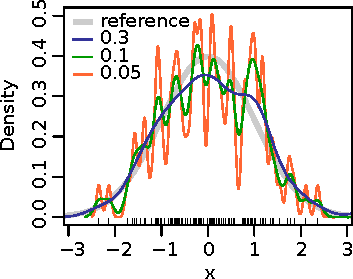
\includegraphics[width=0.5\textwidth]{KDE_example.pdf}
	\caption[Example KDE with different smoothing]{\textbf{Example KDE with different smoothing.} \cite{kde:example_plot} Kernel density estimation is applied on a data sample with 100 random numbers drawn from a normal distribution (gray curve). The blue, green, and orange curves have different bandwidths.}
	\label{kde:example_1d}	
\end{figure}

The kernel function can be a very distinct function that can in principle describe any probability density. In this parameterization method a Gaussian kernel
\begin{align}
	K(t) = \frac{1}{\sqrt{2\pi}}e^{-\frac{1}{2}t^2}
\end{align}
is used.

In order to get the KDE describing the probability density appropriately, one has to choose a reasonable bandwith for the given data sample size. As shown in figure \ref{kde:example_1d}, too low bandwith results in a spiky, fluctuating KDE. If the bandwidth is too high, one might get a rather inaccurate estimator. Therefore it seems reasonable to choose different bandwidth in regions with different amount of statistics which then is called \textit{adaptive} kernel density estimation. \cite{kde:schoenen, kde:wangwang}

\subsection{Adaptive KDE with Gaussian Kernel}
As one can see in the simulation results (cf. \todo{verweis zu map}) and in figure \ref{kde:example_scatter}, each pixel has a certain region of photon directions where it is efficient. However, each pixel is almost \enquote{blind} for most other directions. This results in statistically stable -- \enquote{dense} -- regions but also \enquote{sparse} regions dominated by scattered photons that undergo large statistical fluctuations. Thus, and based on the former conclusions, an approach to adapt the bandwidth to the local statistics should perform well. In this thesis, an algorithm presented by \textsc{B. Wang} and \textsc{X. Wang} in \cite{kde:wangwang} which has been implemented within the scope of \cite{kde:schoenen} is used. The adaptive (in principle weighted) kernel density estimator is calculated by \cite{kde:schoenen,kde:wangwang}
\begin{align}
	f(\vec{x}) = \sum_{i=0}^{n} \frac{w_i}{N_i}e^{-\frac{1}{2}(\vec{x}-\vec{X_i})^T \frac{1}{h\lambda_i} \mathbf{C}^{-1} (\vec{x}-\vec{X_i})}\,,
\end{align}
with
\begin{vardescription}
	n & total number of data points,\\
	w_i & weight of th $i$-th data point,\\
	N_i & Gaussian normalization,\\
	\vec{X_i} & coordinate vector of the $i$-the data point,\\
	h & global bandwidth factor,\\
	\lambda_i & local bandwidth factor,\\
	\mathbf{C} & covariance matrix.\\
\end{vardescription}
The global bandwidth factor $h$ is calculated by the \textit{Silverman rule} \cite{kde:schoenen,kde:wangwang}
\begin{align}
	h = \left(\frac{n(d+2)}{4}\right)^{-\frac{1}{d+4}}\,,
\end{align}
where $d$ equals the number of dimensions of the data (here $d=2$). The local bandwidth $\lambda_i$ is the factor where the local statistics of each data point comes in. It is defined as \cite{kde:schoenen,kde:wangwang}
\begin{align}
	\lambda_i = \left(\frac{\hat{f}(\vec{X_i})}{g}\right)^{-\alpha}\,,
\end{align}
with
\begin{vardescription}
	\hat{f}(\vec{X_i}) = f(\vec{X_i})|_{w_i=\lambda_i=1}\,,\\
	\ln{g} = n^{-1} \sum_{i=0}^{n} \ln{\hat{f}(\vec{X_i})}\,,\\
	\alpha\in[0,1]\,.
\end{vardescription}
For the IceAct parameterization the sensitivity parameter $\alpha$ is set to $\alpha=\num{0.3}$, since this has been shown to be an appropriate value as well as in \cite{kde:schoenen}. Additionally, all $n$ photon hits have the same weight, which results in \cite{kde:schoenen,kde:wangwang}
\begin{align}
	w_i = \frac{1}{n}\,.
\end{align}
To get an idea of the given data points for which the KDE should be calculated, figure \ref{kde:example_scatter} shows a scatter plot of detected photons for an arbitrary camera pixel in a possible range of wavelengths. The need for an adaptive KDE approach is clearly visible by regions with very different statistical densities. In addition, figure \ref{kde:comparison} shows strinkingly the difference between an adaptive and a non-adaptive KDE.

\begin{figure}[h]
	\centering
	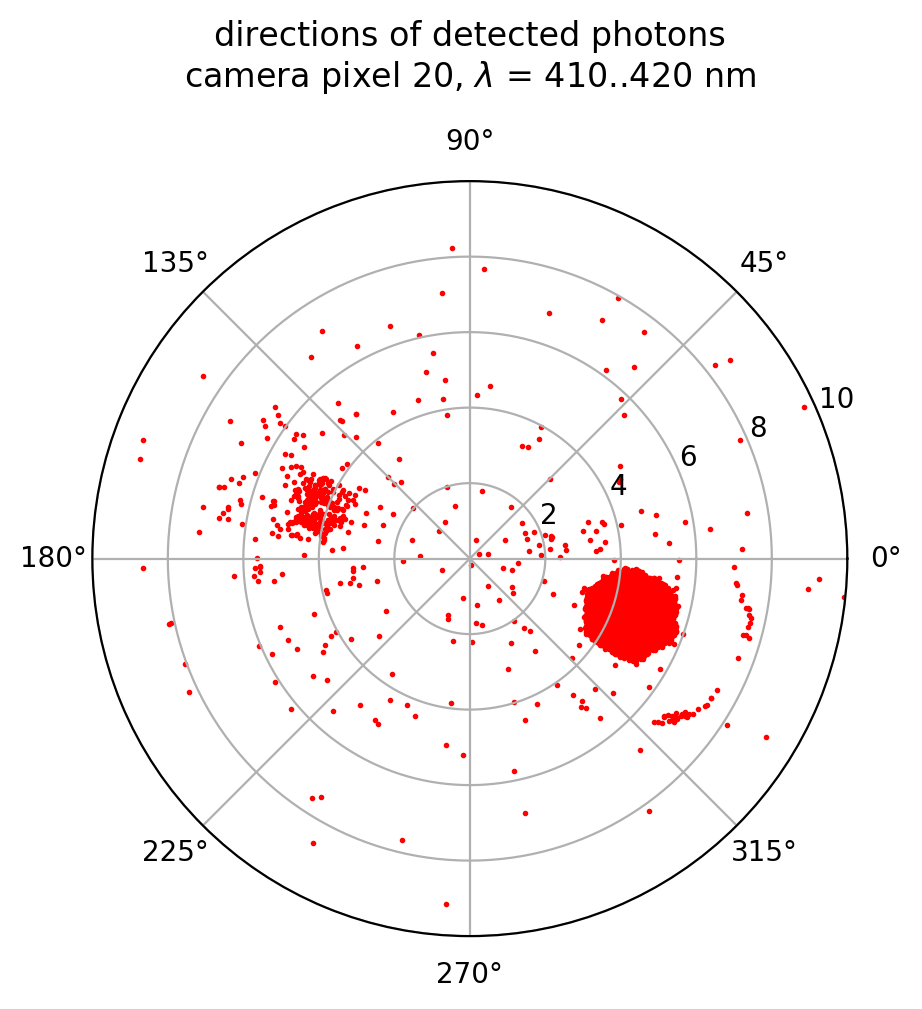
\includegraphics[width=0.5\textwidth]{scatter_px20_wvl410-420nm.png}
	\caption[Example: directions of detected photons as a scatter plot]{\textbf{Example: directions of detected photons as a scatter plot.} A subset of simulated photon directions that are detected in camera pixel 20 with wavelengths between \SI{410}{\nano\meter} and \SI{420}{\nano\meter} are shown in a polar plot. One can clearly see that there are regions with high and low statistical significance.}
	\label{kde:example_scatter}	
\end{figure}

\begin{figure}[h]
	\centering
	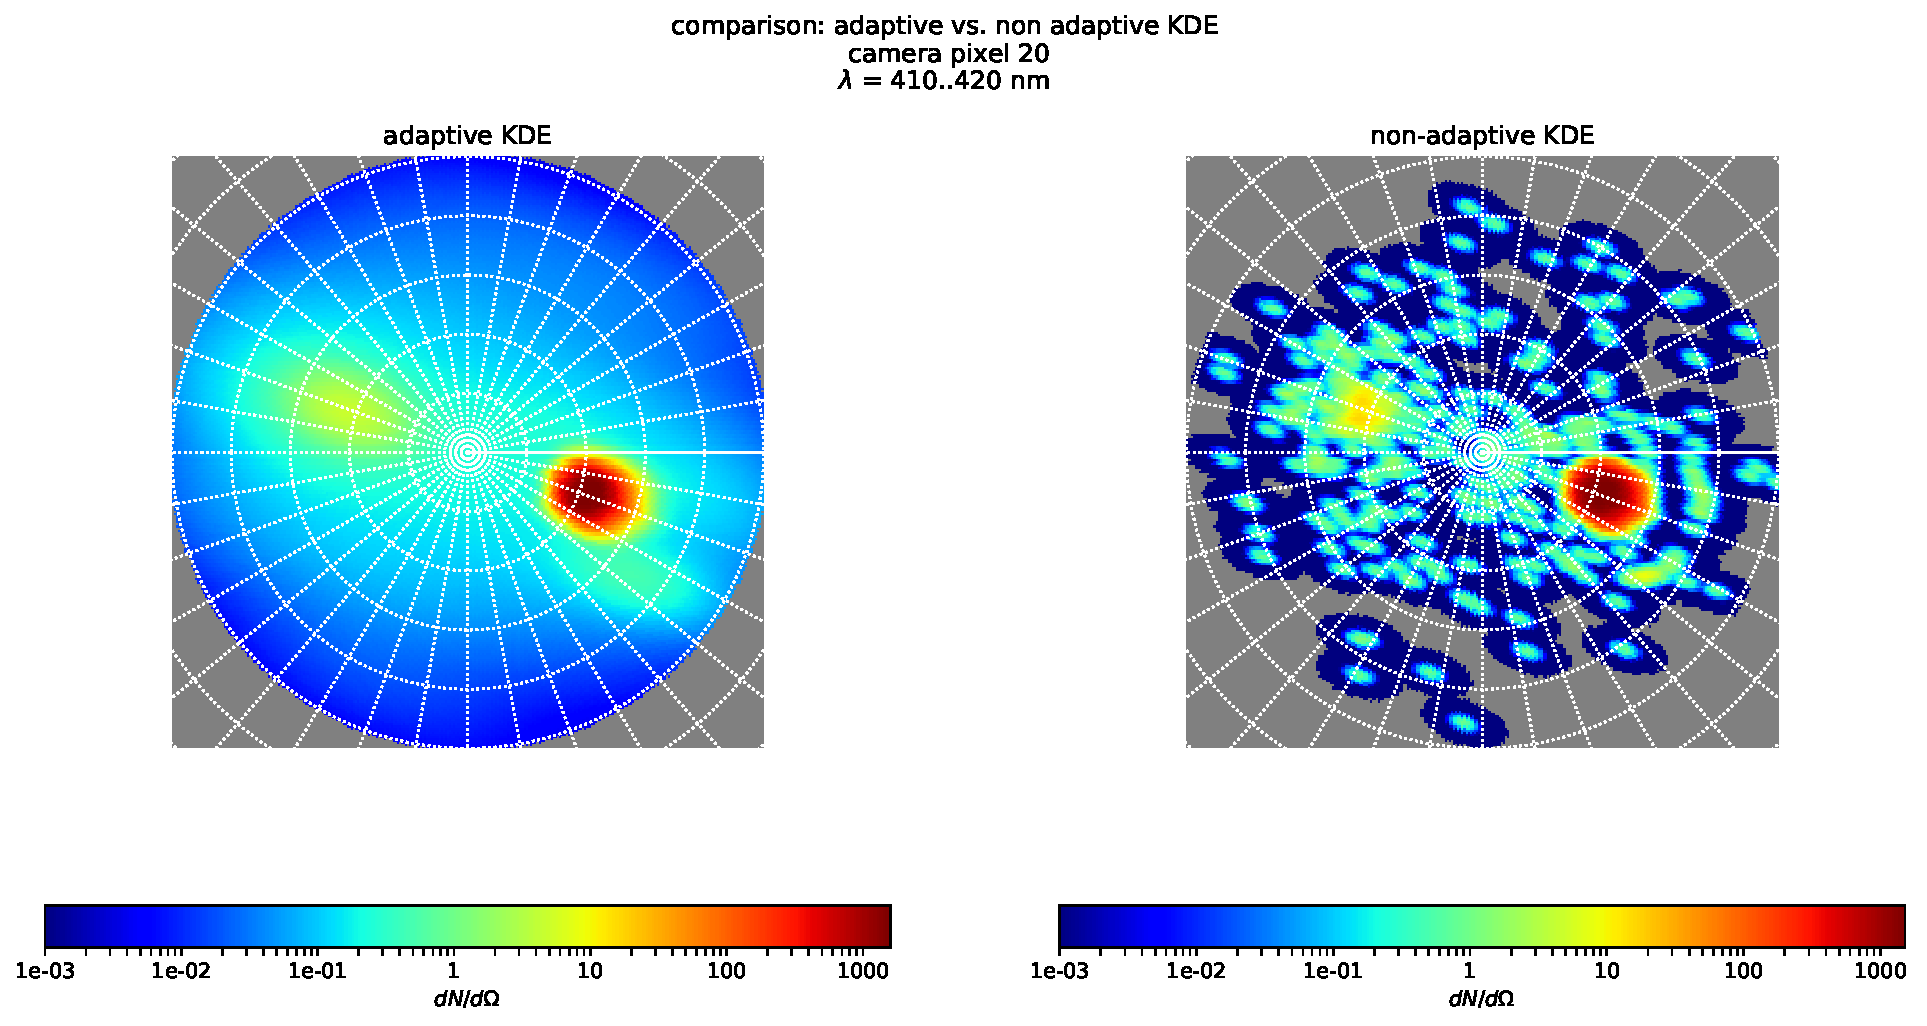
\includegraphics[width=\textwidth]{comparison_adaptive_nonadaptive.pdf}
	\caption[Comparison: adaptive vs. non-adaptive KDE]{\textbf{Comparison: adaptive vs. non-adaptive KDE.} The difference between an adaptive (left) and non-adaptive (right) KDE approach is visible. Especially in the region with low statistics, the non-adaptive KDE is dominated by the fluctuations.}
	\label{kde:comparison}	
\end{figure}

\subsection{Bootstrapping}
One problem of kernel density estimation 

\section{Detection Efficiency}

\subsection{The HEALPix Algorithm}

In order to account for the spherical shape of the angles of incidence it is useful to have angular bins with equal areas. Therefore, in this parameterization method, the \textit{HEALPix} (\textbf{H}ierarchical \textbf{E}qual \textbf{A}rea iso\textbf{L}atitude \textbf{Pix}elization) algorithm is used. It allows a uniform pixelization of incidence angles to the telescope.\\

\todo{healpix pixelization image}

The basic idea is to subdivide the sphere into 12 quadrilateral panes which can then further divided into more sub-panes as shown in figure \todo{figure reference}. A parameter $k$ numbers the subdivision step so that the number of sub-panes per each of the 12 panes is $N_{\text{side}}^2=\left(2^k\right)^2$. Hence, the total amount of pixels on the sphere is then
\begin{align}
N_\text{pix} = 12N_\text{side}^2\,.
\end{align}
Obviously, the angular resolution is dependent on $N_\text{pix}$, henceforth referred to as \enquote{pixel}.

\begin{table}[h]
\centering
\begin{tabular}{S[table-format=2.0]|S[table-format=4.0]|S[table-format=9.0]|S[table-format=2.2]}
\multicolumn{1}{l|}{$k$} & \multicolumn{1}{l|}{$N_\text{side} = 2^k$} & \multicolumn{1}{l|}{$N_\text{pix} = 12N_\text{nside}^2$} & \multicolumn{1}{l}{$\theta_\text{pix}$} \\
\hline
0  & 1    & 12        &  \SI{58.6}{\degree}\\
1  & 2    & 48        &  \SI{29.3}{\degree}\\
2  & 4    & 192       &  \SI{14.7}{\degree}\\
3  & 8    & 768 	  &  \SI{7.33}{\degree}\\
4  & 16   & 3072      &  \SI{3.66}{\degree}\\
5  & 32   & 12288     &  \SI{1.83}{\degree}\\
6  & 64   & 49152     &  \SI{55.0}{\arcminute}\\
7  & 128  & 196608    &  \SI{27.5}{\arcminute}\\
8  & 256  & 786432    &  \SI{13.7}{\arcminute}\\
9  & 512  & 3145728   &  \SI{6.87}{\arcminute}\\
10 & 1024 & 12582912  &  \SI{3.44}{\arcminute}\\
11 & 2048 & 50331648  &  \SI{1.72}{\arcminute}\\
12 & 4096 & 201326592 &  \SI{51.5}{\arcsecond}\\
13 & 8192 & 805306368 &  \SI{25.8}{\arcsecond}\\
\multicolumn{1}{c|}{\vdots} & \multicolumn{1}{c|}{\vdots} & \multicolumn{1}{c|}{\vdots} & \multicolumn{1}{c}{\vdots} \\
\end{tabular}
\caption[HEALPix parameters and resulting angular resolutions]{\textbf{HEALPix parameters and resulting angular resolutions.} $k$ represents the number of dividing iterations on the 12 panes, $N_\text{side}$ the number of tiles per pane edge, $N_\text{pix}$ the total number of pixels, and $\theta_\text{pix}$ the angular resolution defined by the angular length of a pixel edge. \cite{healpix:paper}}
\end{table}

For the application in this simulation the pixelization of a whole sphere is not needed since the telescope only has a field of view of about \SI{12}{\degree} (i.e. $\theta \leq \SI{6}{\degree}$). Considering that, one only needs a smaller sector of pixels around the zenith at $\theta = \SI{0}{\degree}$ which reduces the number of needed HEALPix by a factor of
\begin{align}
	\Gamma = \frac{1}{4\pi}\int\limits_{0}^{2\pi}\int\limits_{0}^{\theta_\text{max}}\sin{\theta} d\theta d\phi = \frac{1-\cos\theta_\text{max}}{2}\,.
\end{align}
For the IceAct simulation with $\theta_\text{max} = \SI{10}{\degree}$ this leads to the fact that only about \SI{0.76}{\percent} of the HEALPixes are needed.

\section{Lookup Table}

\section{CORSIKA Implementation}\todo{vermutlich quatsch}
